%
% $RCSfile: model.tex,v $
%
% Copyright (c) 2001-2004. Christian Heller. All rights reserved.
%
% No copying, altering, distribution or any other actions concerning this
% document, except after explicit permission by the author!
% At some later point in time, this document is planned to be put under
% the GNU FDL license. For now, _everything_ is _restricted_ by the author.
%
% http://www.cybop.net
% - Cybernetics Oriented Programming -
%
% http://www.resmedicinae.org
% - Information in Medicine -
%
% @author Christian Heller <christian.heller@tuxtax.de>
%

\subsection{Model}
\label{model_heading}

A theoretical \emph{Model} is an abstract clip of the real world, and exists in
the human mind. Another common word for \emph{Model} is \emph{Concept}.
It is the subsumption of \emph{Item}, \emph{Category} and \emph{Compound},
resulting from the three activities of abstraction: \emph{Discrimination},
\emph{Categorization} and \emph{Composition}. As such, each model knows about
its super model and the parts it consists of (figure \ref{abstract_model_figure}).
Software developers would call the illustration of these relations a \emph{Schema}
or \emph{Meta Model}.

\begin{figure}[ht]
    \begin{center}
        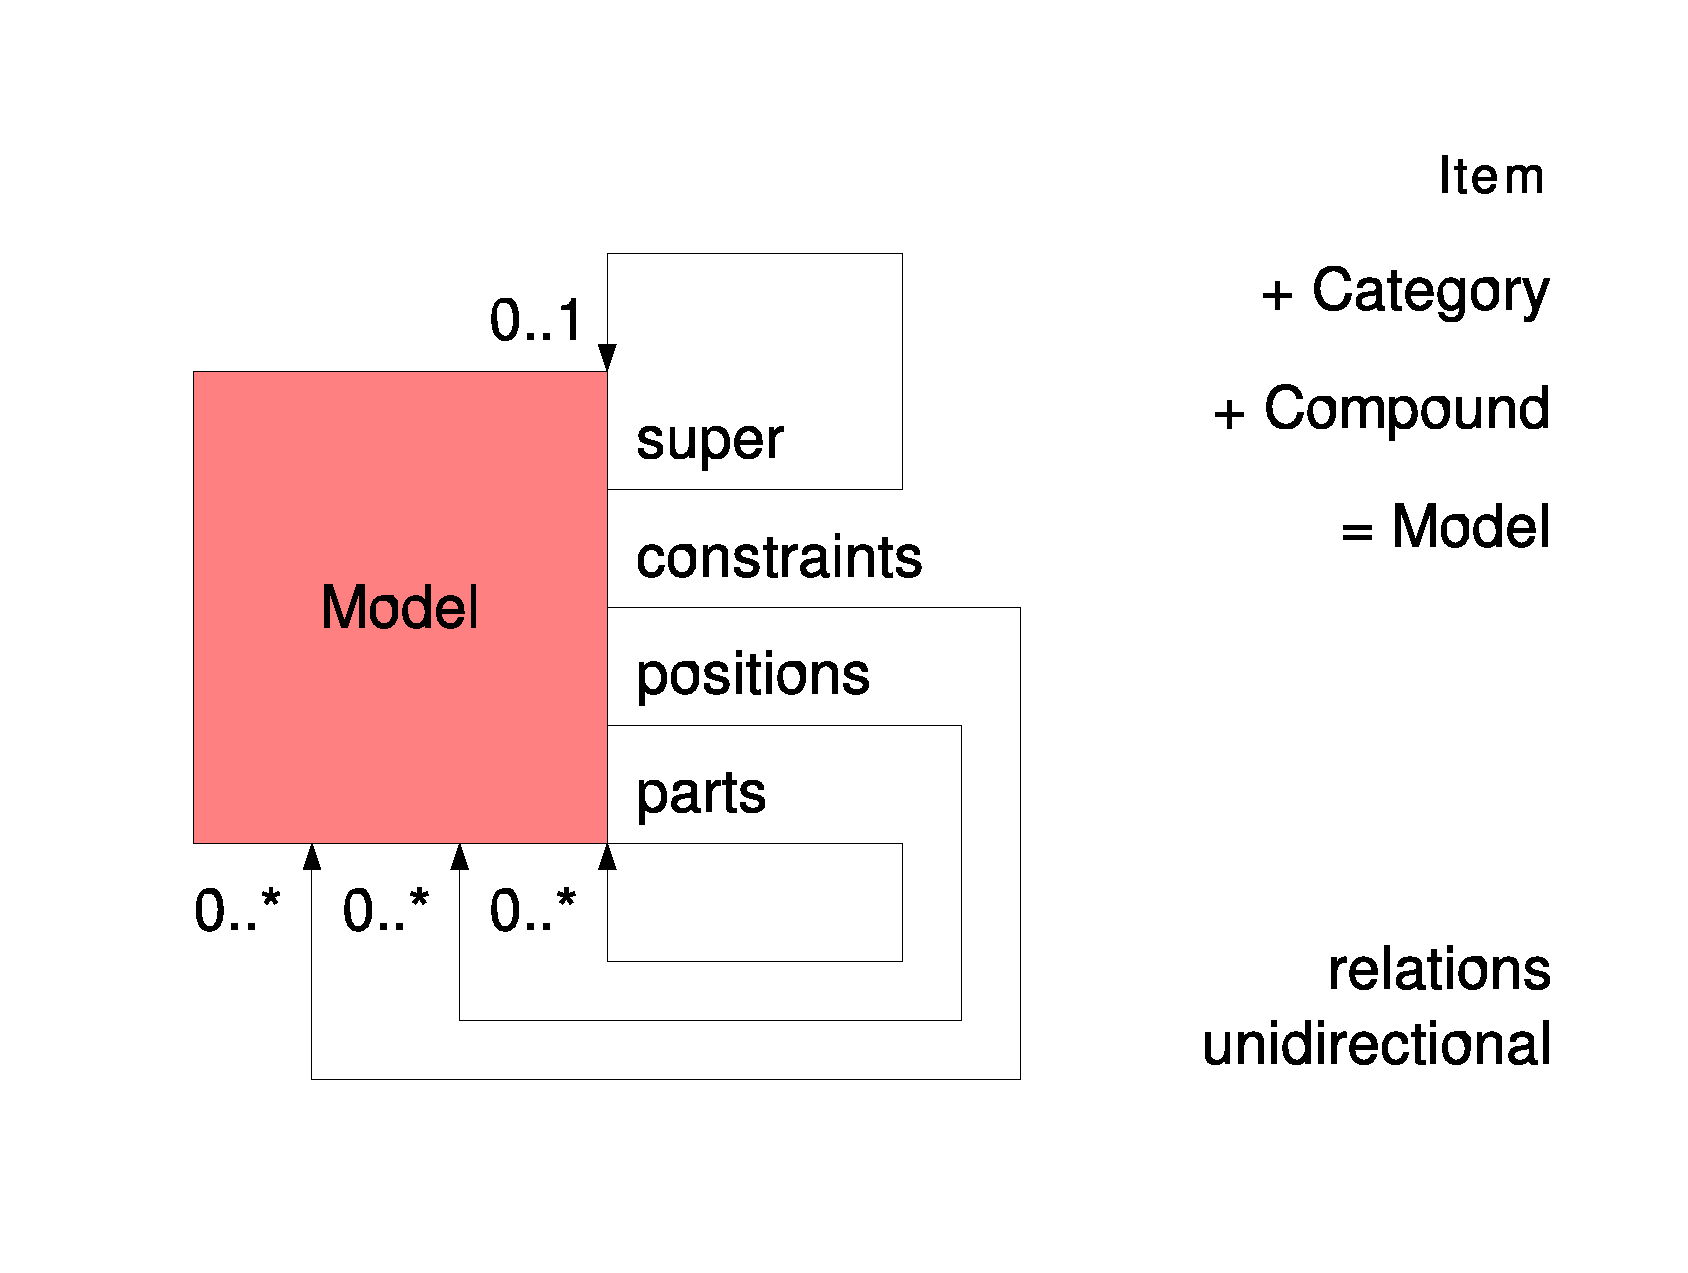
\includegraphics[scale=0.3]{vector/abstract_model.eps}
        \caption{Model as subsumption of Item, Category, Compound}
        \label{abstract_model_figure}
    \end{center}
\end{figure}
